%!TEX root = karen.tex

\chapter{Keeneland Benchmarks}
\label{app:keeneland_alltoallv_benchmarks}

The benchmarks in our first paper (\cite{BolligFlyerErlebacher2012}) demonstrated the initial scaling of the implementation for a distributed RK4 iteration using primitive blocking MPI\_Send/MPI\_Recv communication routines. The collective was a round-robin all-to-subset connection between processors, each taking a turn to send data (0 or more bytes) or otherwise wait to receive data. Blocking communication was implemented for code verification, and the linear-in-$x$ partitioning was employed. Benchmarks in \cite{BolligFlyerErlebacher2012} were acquired on the multi-GPU cluster named Keeneland \cite{Vetter2011}. 

The implementation demonstrated poor scaling behavior as blocking collectives serialized transmissions, and every process had to wait until the end of the collective to proceed. The objective in \cite{BolligFlyerErlebacher2012}, however, was not to present a well tuned distributed GPU implementation of RBF-FD. Instead we focused on the design decisions for partitioning, index mapping, etc. and verification of both single and distributed GPU implementations as inefficient as they were. 


This appendix provides new data from Keeneland for direct comparison with \cite{BolligFlyerErlebacher2012}.

%was similarly acquired on the Keeneland GPU cluster but tests the MPI\_Alltoallv collective. It is provided for comparison with \cite{BolligFlyerErlebacher2012}.

\section{Single GPU SpMV on Keeneland} 

%TODO: cleanup this section
\authnote{FIX UP}

An SpMV requires $N * n * 2$ floating point operations due to the 2 operations, multiply and add, required when applying $N$ dot-products of size $n$. An iteration of RK4 requires four evaluations of the function $F(t,\vu)$, whose operation count varies by application, plus $7*N$ operations (four additions and three multiplications) per time-step. 

In Figures~\ref{fig:gflops_cpu_1proc_keeneland}, \ref{fig:gflops_gpu_1proc_oneWarp_keeneland} and \ref{fig:gflops_gpu_1proc_oneThread_keeneland}, each function evaluation in the RK4 performs three independent SpMVs and two AXPY operations ($2*N$ each) for a total of $6*N*n + 4*N$ operations. Thus the total operation count for a single RK4 iteration is estimated at: $24*N*n +23*N$. 
For Vortex Roll-up, only two SpMVs and one AXPY are required, which drops the total operation count to: $16*N*n + 15*N$. 

Figure~\ref{fig:gflops_cpu_1proc_keeneland} provides the GFLOP/sec for Cosine Bell Advection on the Keeneland GPU cluster for a single CPU running the nested loop evaluation, optimized with auto-vectorization and auto-blocking provided by the Intel compiler. Figure~\ref{fig:gflops_gpu_1proc_oneWarp_keeneland} and \ref{fig:gflops_gpu_1proc_oneThread_keeneland} show the GFLOP/sec achieved by our custom GPU kernels running on the M2070 GPUs. The corresponding speedups achieved in each case over the CPU is provided in Figures~\ref{fig:speedup_1proc_oneWarp_keeneland} and \ref{fig:speedup_1proc_oneThread_keeneland}. 

\begin{figure}
\centering
\begin{subfigure}[t]{0.425\textwidth}
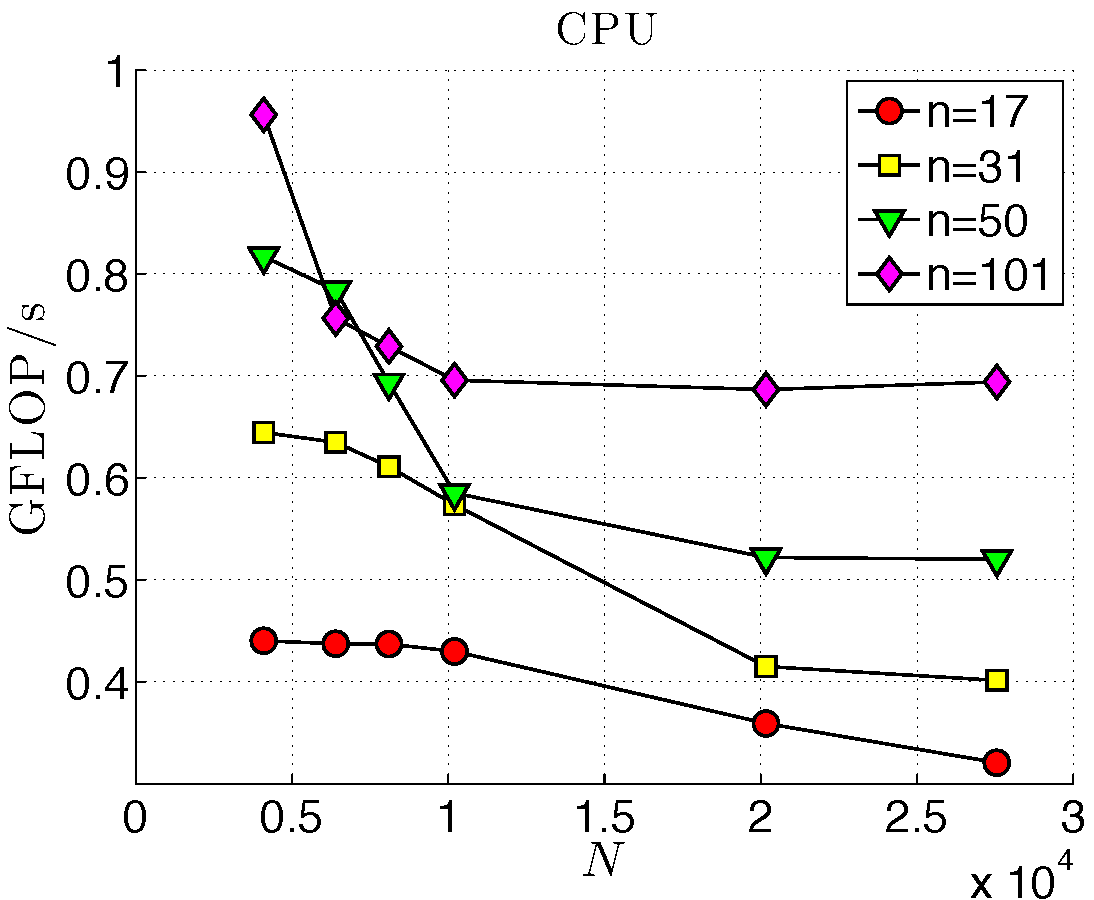
\includegraphics[width=\textwidth]{../figures/keeneland_results/alltoallv_cosine/gflops_cpu_1proc_oneWarpPerStencil.pdf}
\caption{One warp per stencil kernel on one GPU in Keeneland}
\label{fig:gflops_cpu_1proc_keeneland}
\end{subfigure} \\
\begin{subfigure}[t]{0.425\textwidth}
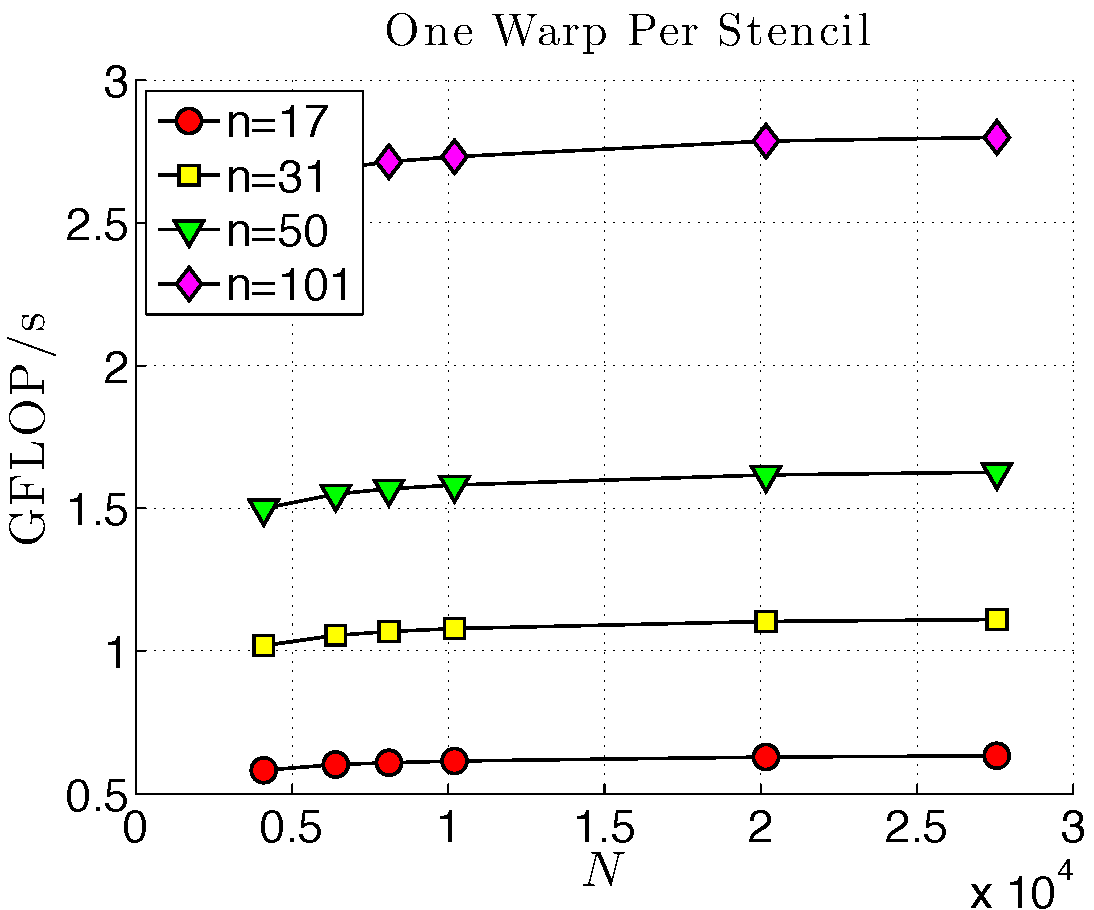
\includegraphics[width=\textwidth]{../figures/keeneland_results/alltoallv_cosine/gflops_gpu_1proc_oneWarpPerStencil.pdf}
\caption{One warp per stencil kernel on one GPU in Keeneland}
\label{fig:gflops_gpu_1proc_oneWarp_keeneland}
\end{subfigure} 
\quad
\begin{subfigure}[t]{0.425\textwidth}
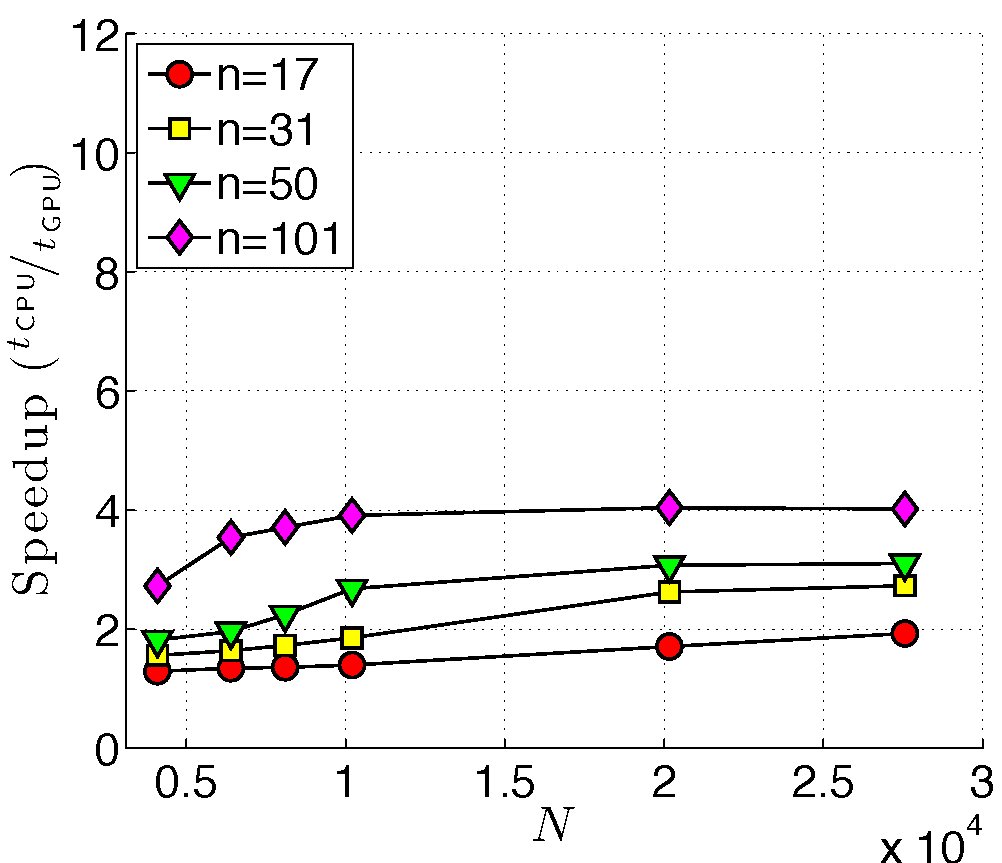
\includegraphics[width=\textwidth]{../figures/keeneland_results/alltoallv_cosine/speedup_1proc_oneWarpPerStencil.pdf}
\caption{One warp per stencil kernel on one GPU in Keeneland}
\label{fig:speedup_1proc_oneWarp_keeneland}
\end{subfigure} 
\begin{subfigure}[t]{0.425\textwidth}
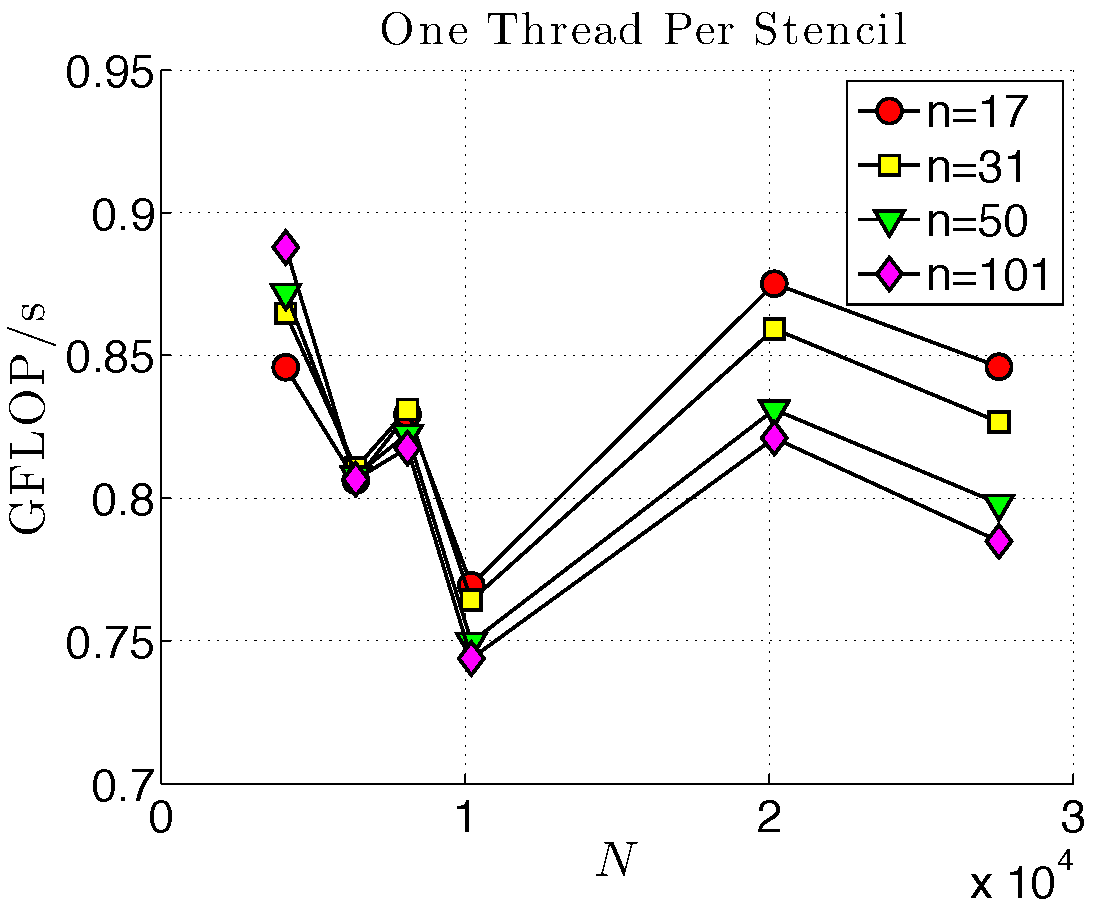
\includegraphics[width=\textwidth]{../figures/keeneland_results/alltoallv_cosine/gflops_gpu_1proc_oneThreadPerStencil.pdf}
\caption{One warp per stencil kernel on one GPU in Keeneland}
\label{fig:gflops_gpu_1proc_oneThread_keeneland}
\end{subfigure}
\quad
\begin{subfigure}[t]{0.425\textwidth}
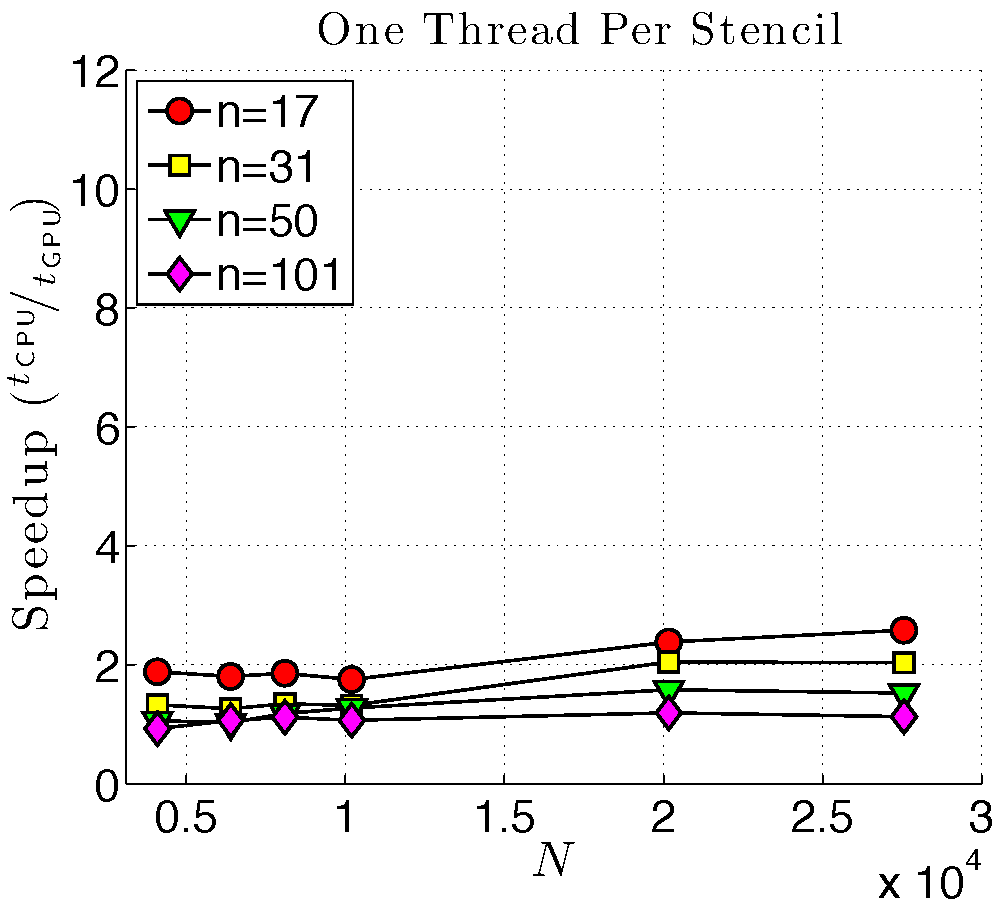
\includegraphics[width=\textwidth]{../figures/keeneland_results/alltoallv_cosine/speedup_1proc_oneThreadPerStencil.pdf}
\caption{One warp per stencil kernel on one GPU in Keeneland}
\label{fig:speedup_1proc_oneThread_keeneland}
\end{subfigure} 
\caption{Benchmarks from the Keeneland GPU cluster compare the average run-time of a single time-step of RK4 executed custom kernels.}
\end{figure} 

\section{Keeneland Scaling with MPI\_Alltoallv}

The following data demonstrates performance of the implementation with an MPI\_alltoallv collective. The benchmarks test the cosine bell advection from Section~\ref{sec:cosine_bell}. 

Figure~\ref{fig:alltoall_multicpu_scaling} shows the strong scalability of our method on multiple CPUs. This figure demonstrates that our method does scale linearly (almost super-linearly) as the number of CPUs increases. 
%, so our prospect for spanning all CPUs on Keeneland is within reach for problem sizes large enough.
The super-linear speedup is due to improved caching on processors as individual problem sizes decrease and the processors are able to keep a larger percentage of the problem within fast cache memory.

\begin{figure}
\centering
\begin{subfigure}[t]{0.425\textwidth}
\centering
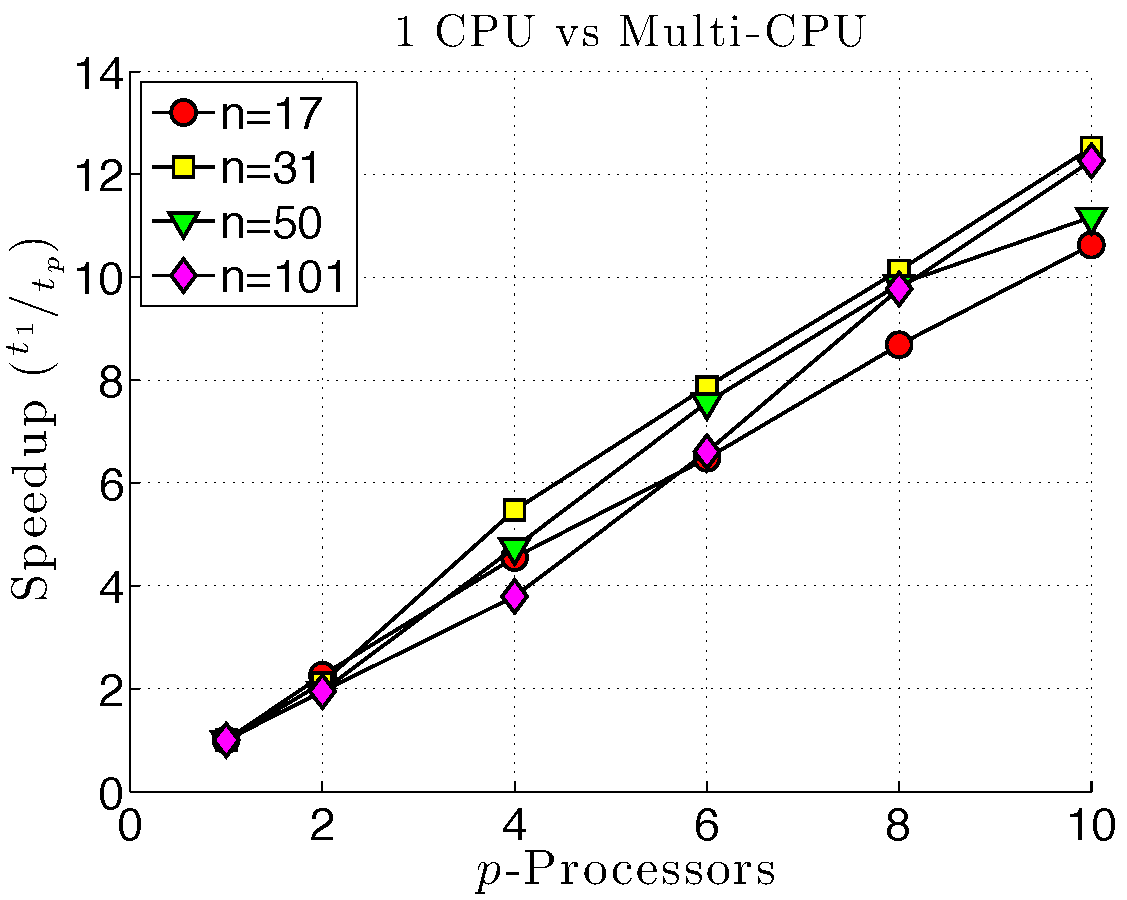
\includegraphics[width=1.0\textwidth]{../figures/keeneland_results/alltoallv_cosine/speedup_1CPU_vs_NCPU.pdf}
\caption{Multi-CPU strong scaling on Keeneland for one warp per stencil. Problem size is sufficiently large to hide latency in MPI communication.}
\label{fig:alltoall_multicpu_scaling}
\end{subfigure} 
\begin{subfigure}[t]{0.425\textwidth}
\centering
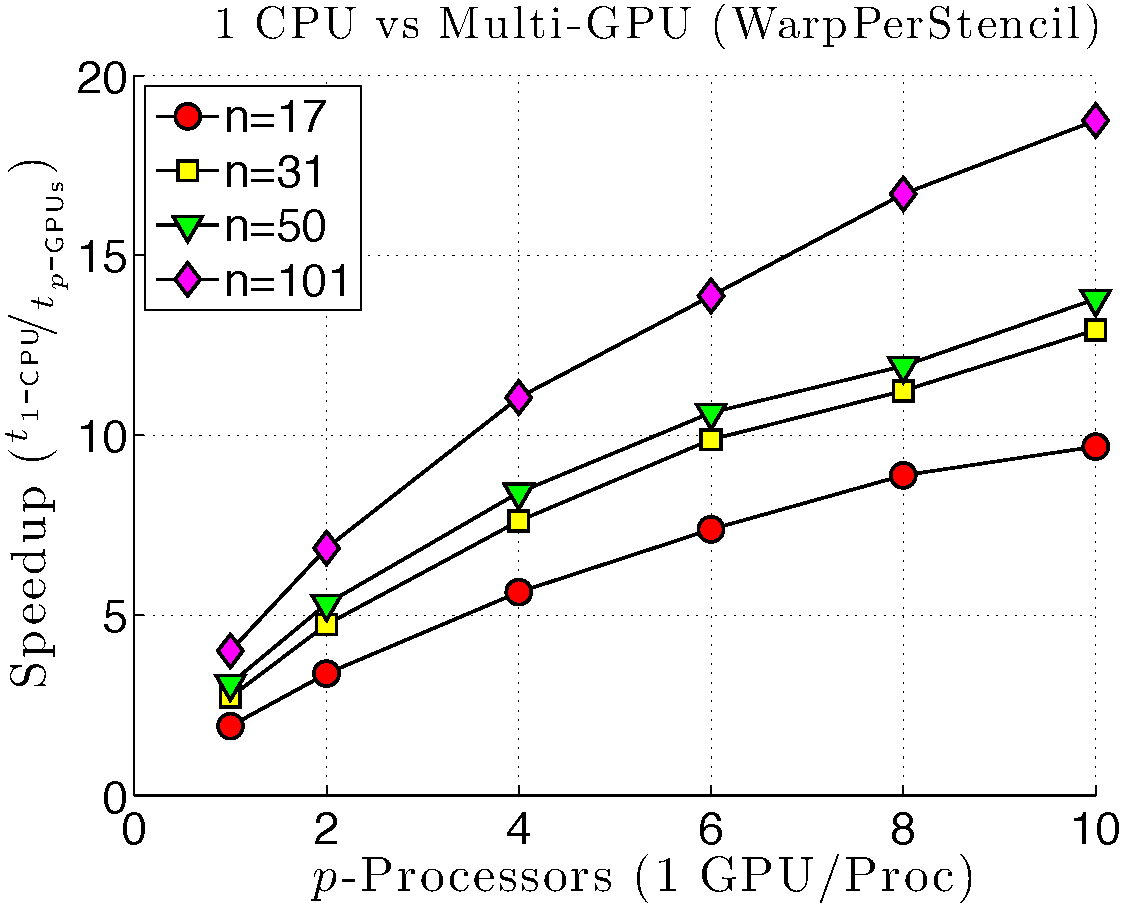
\includegraphics[width=1.0\textwidth]{../figures/keeneland_results/alltoallv_cosine/speedup_1CPU_vs_NGPU_WarpPerStencil.pdf}
\caption{Multi-GPU strong scaling vs one CPU on Keeneland for one warp per stencil}
\label{fig:alltoall_multigpu_vs_cpu_scaling}
\end{subfigure} 
\begin{subfigure}[t]{0.425\textwidth}
\centering
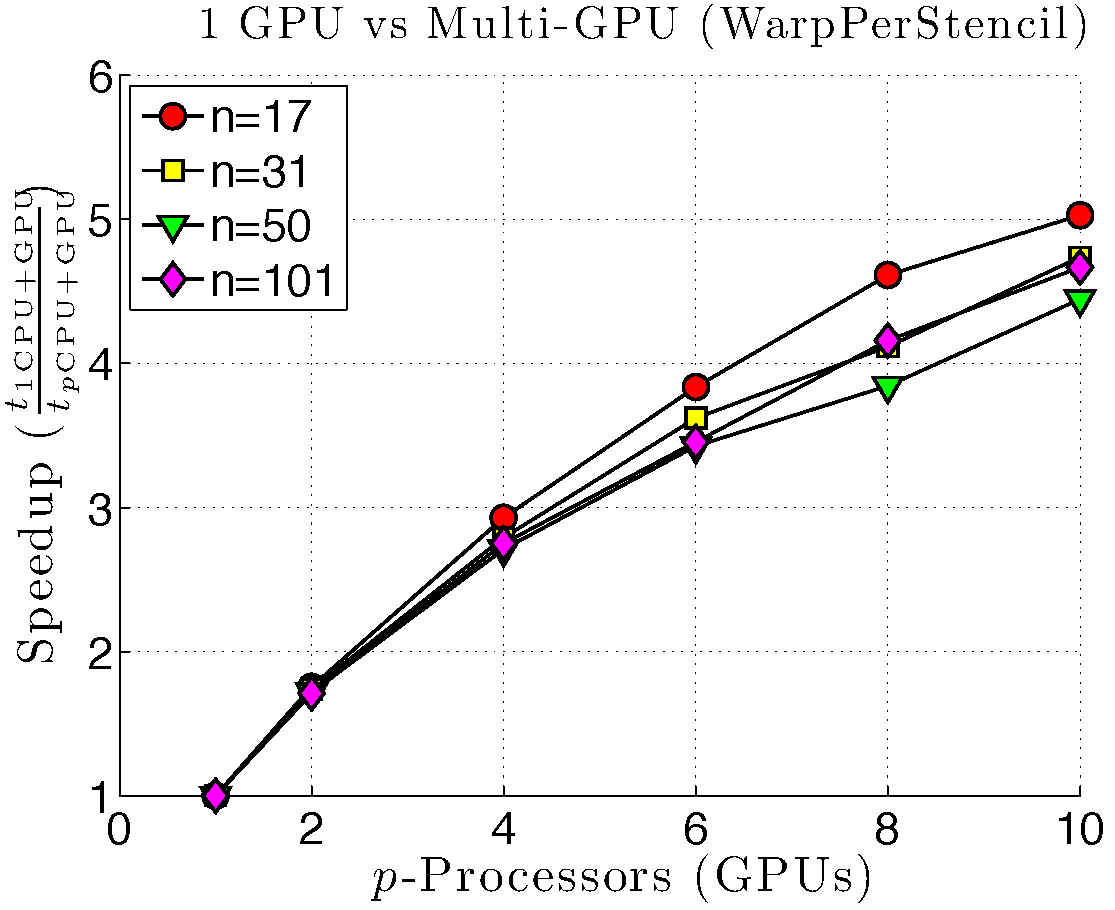
\includegraphics[width=1.0\textwidth]{../figures/keeneland_results/alltoallv_cosine/speedup_1GPU_vs_NGPU_WarpPerStencil.pdf}
\caption{Multi-GPU strong scaling vs one GPU on Keeneland for one warp per stencil}
\label{fig:alltoall_multigpu_vs_gpu_scaling}
\end{subfigure} 
\end{figure}

\begin{figure}
\centering
\begin{subfigure}[t]{0.425\textwidth}
\centering
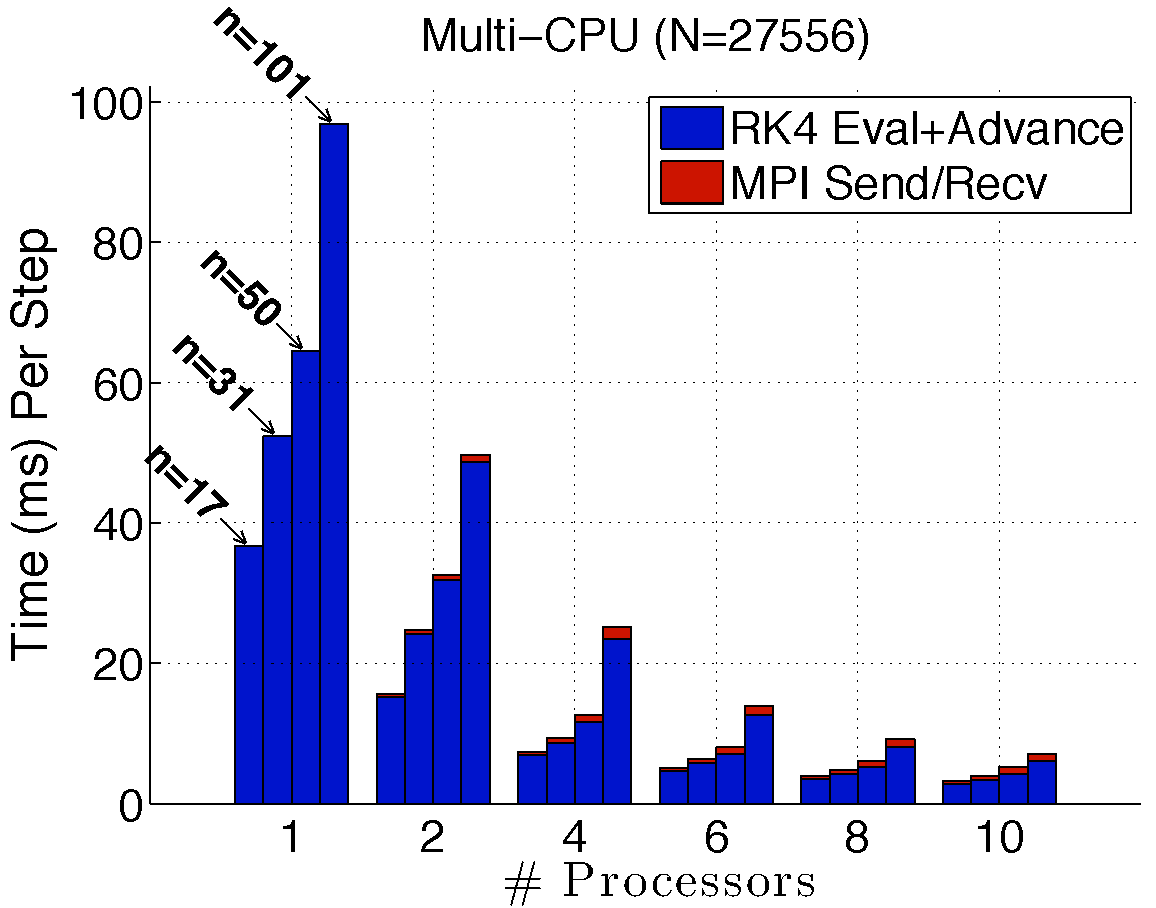
\includegraphics[width=1.0\textwidth]{../figures/keeneland_results/alltoallv_cosine/multiCPU_costs.pdf}
\caption{Multi-CPU}
\label{fig:alltoall_multicpu_costs}
\end{subfigure} 
\begin{subfigure}[t]{0.425\textwidth}
\centering
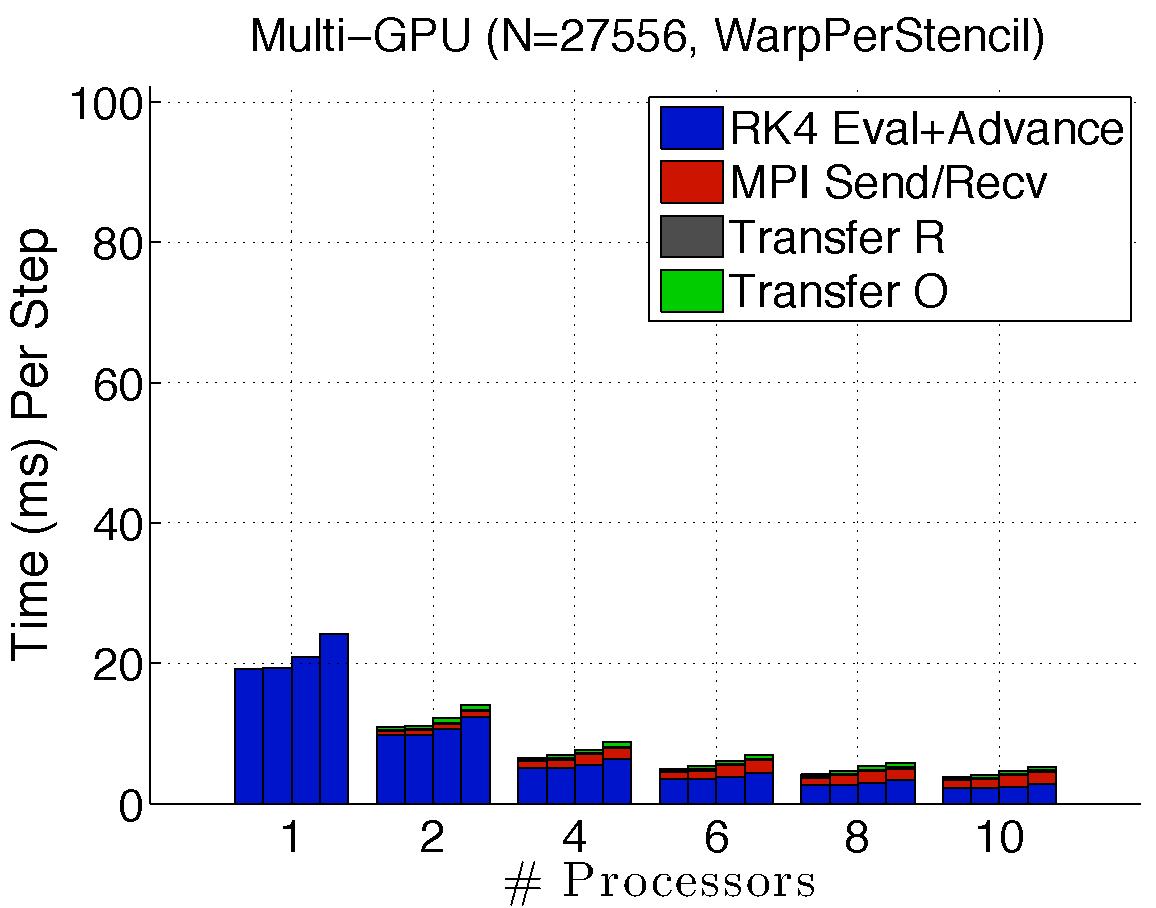
\includegraphics[width=1.0\textwidth]{../figures/keeneland_results/alltoallv_cosine/multiGPU_warp_costs.pdf}
\caption{Multi-GPU}
\label{fig:alltoall_multigpu_costs}
\end{subfigure} 
\caption{Cost comparison of benchmark components on Keeneland. The cost of MPI communication is significantly reduced and allows further scaling. The ``MPI Send/Recv" component represents the time for an MPI\_Alltoallv collective.}
\end{figure} 

Figure~\ref{fig:alltoall_multigpu_vs_cpu_scaling}  shows the scaling of multiple GPUs vs 1 CPU. Ideally, this figure would be the product of the previous two figures since the GPUs are attached to CPUs in a one to one correspondence. However, we see from the sub-linear scaling that while the GPU accelerators are decreasing the time to compute solutions, there is less and less return of investment as the number of processors increase. Between this Figure and the previous, the only thing that differs is the hardware on which stencils are evaluated. The cost of communication stays the same as in the previous figure. But that means the communication consumes a increasing percentage of the iteration time, until is dominates. 
Additionally, computing on the GPU requires transfer (additional communication) of data between CPU and GPU. 

Figure~\ref{fig:alltoall_multigpu_vs_gpu_scaling} shows the scalability of multiple GPUs vs 1 GPU. Here we see a sub-linear behavior for all cases. This is attributed to both the cost of transfer between CPUs and GPUs and the decreasing problem size as number of processors increases, which underutilizes the GPUs. 


Figure~\ref{fig:alltoall_multicpu_costs} and Figure~\ref{fig:alltoall_multigpu_costs} show the smaller percentage of time per iteration dedicated to communication compared to the figures in the paper. In the Figure~\ref{fig:alltoall_multigpu_costs}, the way the times bottom out indicates we are/have converged on the minimum time required to launch a GPU kernel, transfer to/from the GPU, and communicate the problem via MPI. To scale to more processors, a larger problem size is absolutely necessary.





\chapter{Spear Benchmarks} 
\label{app:spear_alltoallv_benchmarks}

The data in this appendix was acquired on the FSU Spear cluster. It is provided for comparison with \cite{BolligFlyerErlebacher2012}.

\section{Spear Scaling with MPI\_Alltoallv}

Although the Spear cluster is not identical to Keeneland, it runs similar GPU hardware allowing for direct comparison


\begin{figure}
\centering
\begin{subfigure}[t]{0.425\textwidth}
\centering
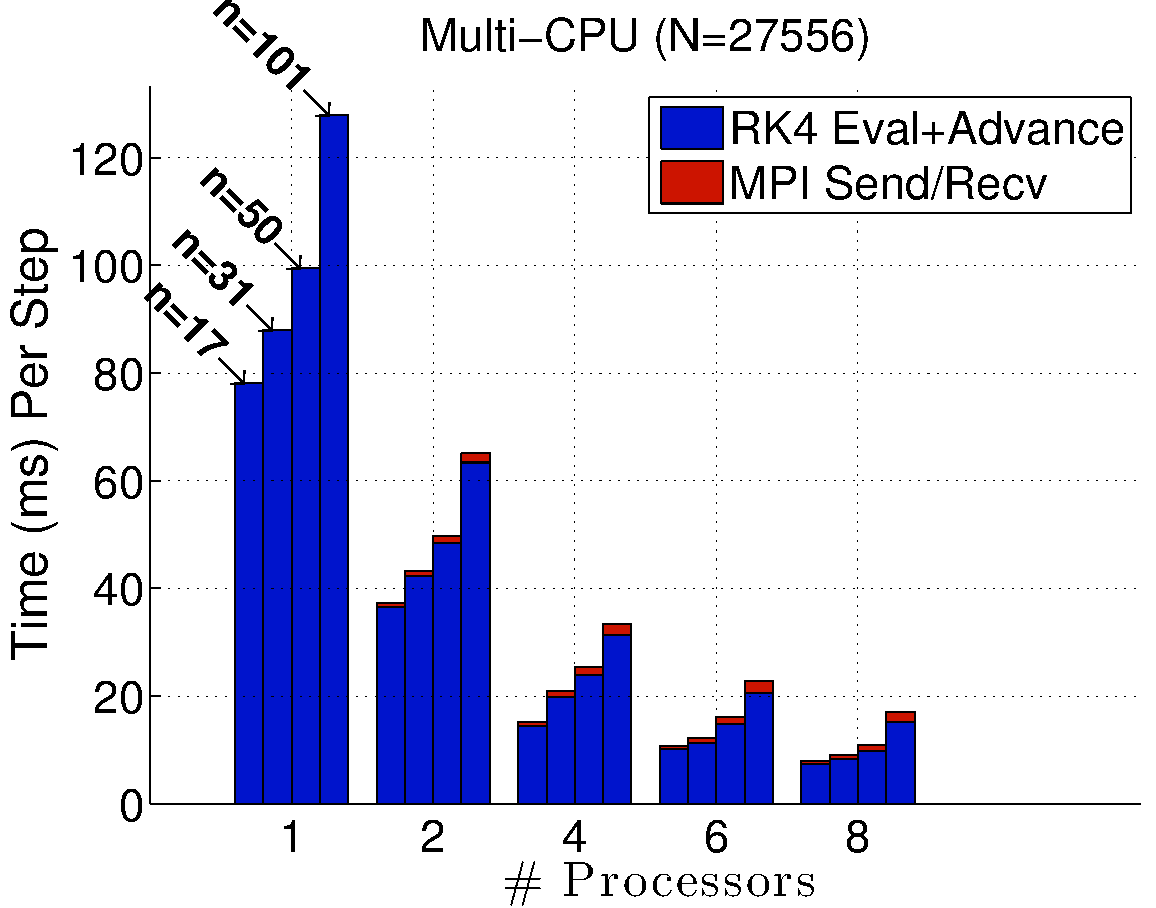
\includegraphics[width=1.0\textwidth]{../figures/spear_results/vortex/multiCPU_costs-eps-converted-to.pdf}
\caption{Multi-GPU strong scaling vs one GPU on Spear for one warp per stencil}
\label{fig:spear_alltoall_multigpu_vs_gpu_scaling}
\end{subfigure} 
\begin{subfigure}[t]{0.425\textwidth}
\centering
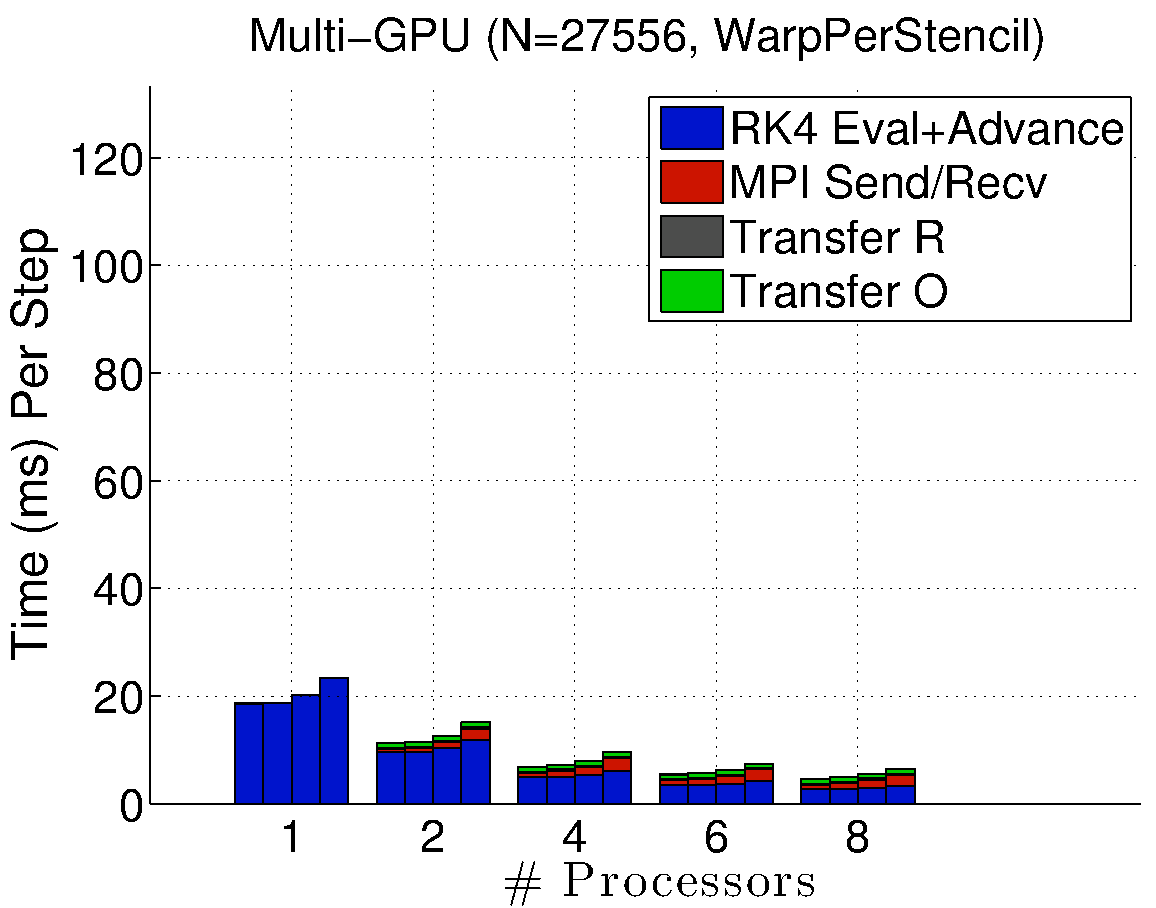
\includegraphics[width=1.0\textwidth]{../figures/spear_results/vortex/multiGPU_warp_costs-eps-converted-to.pdf}
\caption{Multi-GPU strong scaling vs one GPU on Spear for one warp per stencil}
\label{fig:spear_alltoall_multigpu_vs_gpu_scaling}
\end{subfigure} 
%\begin{subfigure}[t]{0.425\textwidth}
%\centering
%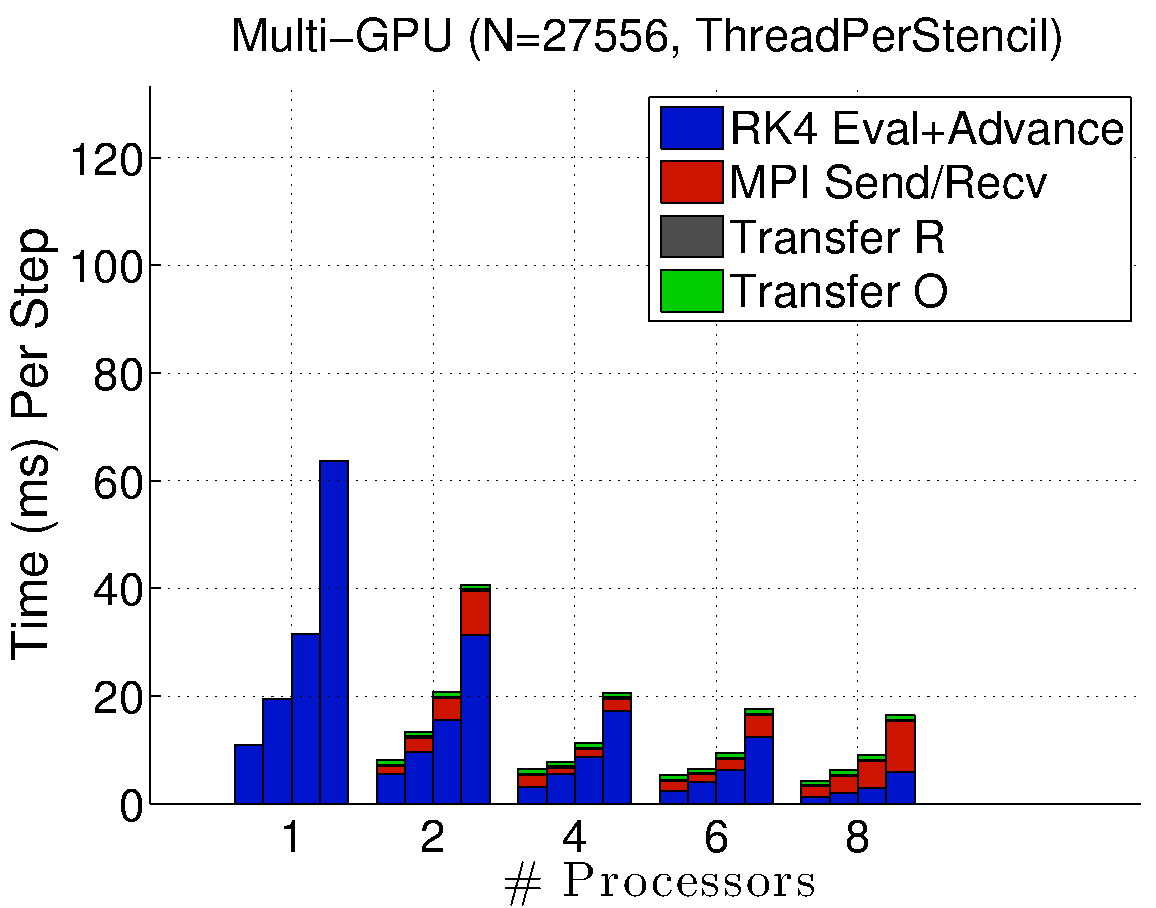
\includegraphics[width=1.0\textwidth]{../figures/spear_results/vortex/multiGPU_thread_costs-eps-converted-to.pdf}
%\caption{Multi-GPU strong scaling vs one GPU on Spear for one thread per stencil}
%\label{fig:alltoall_multigpu_vs_gpu_scaling}
%\end{subfigure} 
\end{figure} 

\begin{figure}
\centering
\begin{subfigure}[t]{0.425\textwidth}
\centering
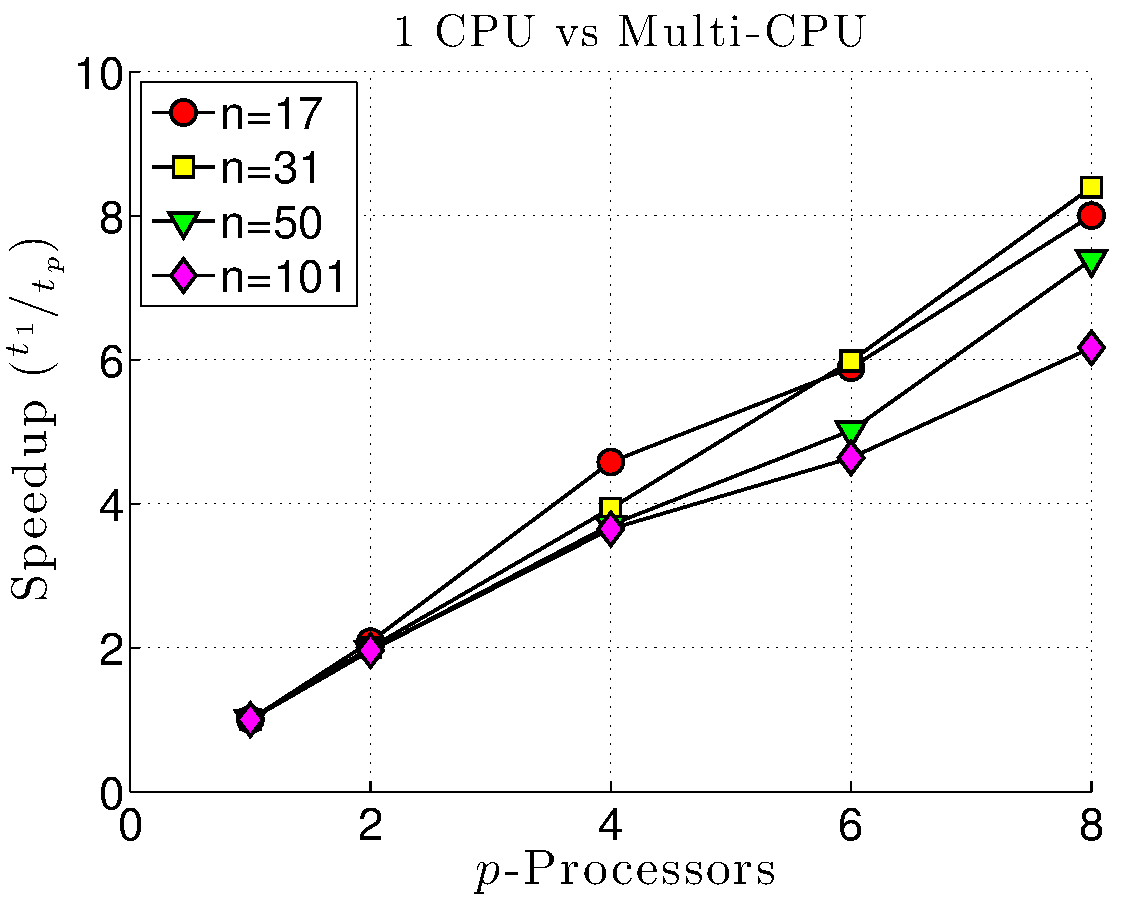
\includegraphics[width=1.0\textwidth]{../figures/spear_results/vortex/speedup_1CPU_vs_NCPU-eps-converted-to.pdf}
\caption{Multi-CPU strong scaling on Spear for one warp per stencil}
\label{fig:spear_alltoall_multicpu_scaling}
\end{subfigure} 
\begin{subfigure}[t]{0.425\textwidth}
\centering
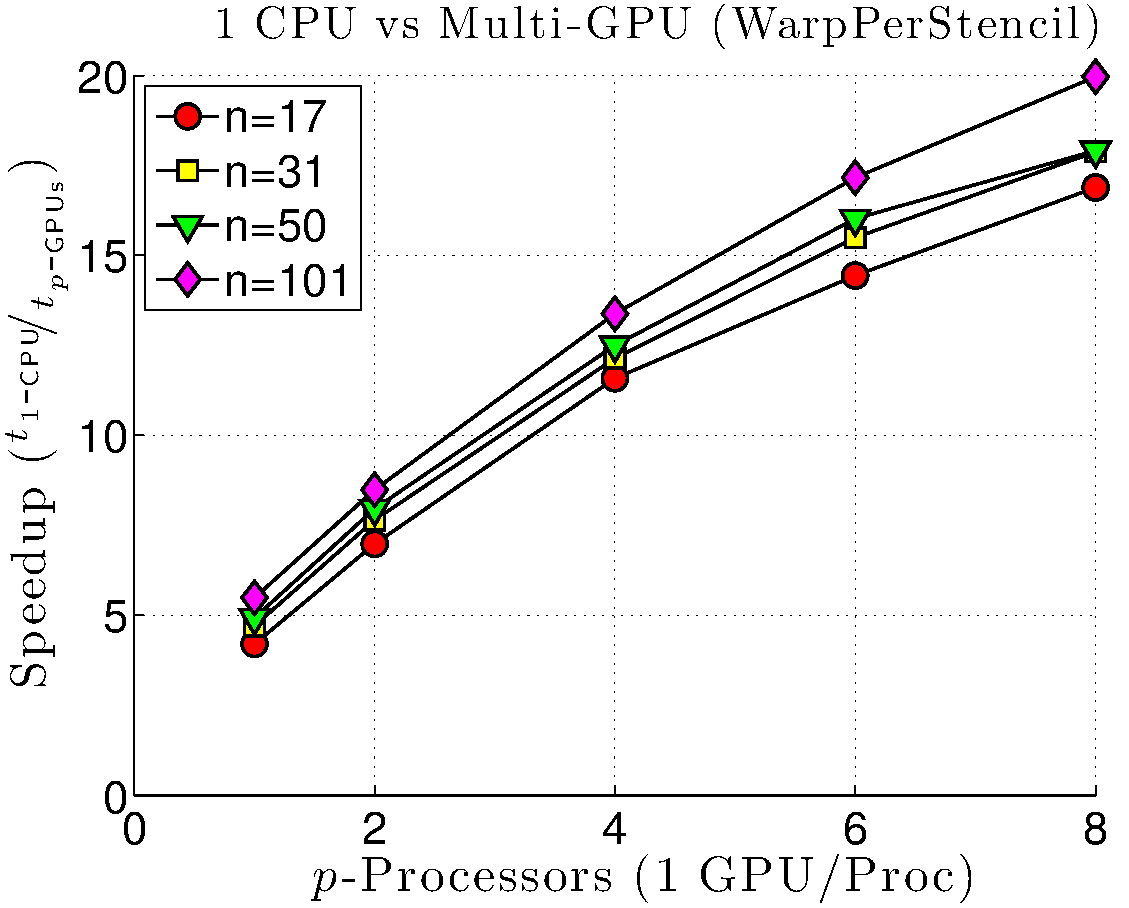
\includegraphics[width=1.0\textwidth]{../figures/spear_results/vortex/speedup_1CPU_vs_NGPU_WarpPerStencil-eps-converted-to.pdf}
\caption{Multi-GPU strong scaling vs one CPU on Spear for one warp per stencil}
\label{fig:spear_alltoall_multigpu_vs_cpu_scaling}
\end{subfigure} 
\begin{subfigure}[t]{0.425\textwidth}
\centering
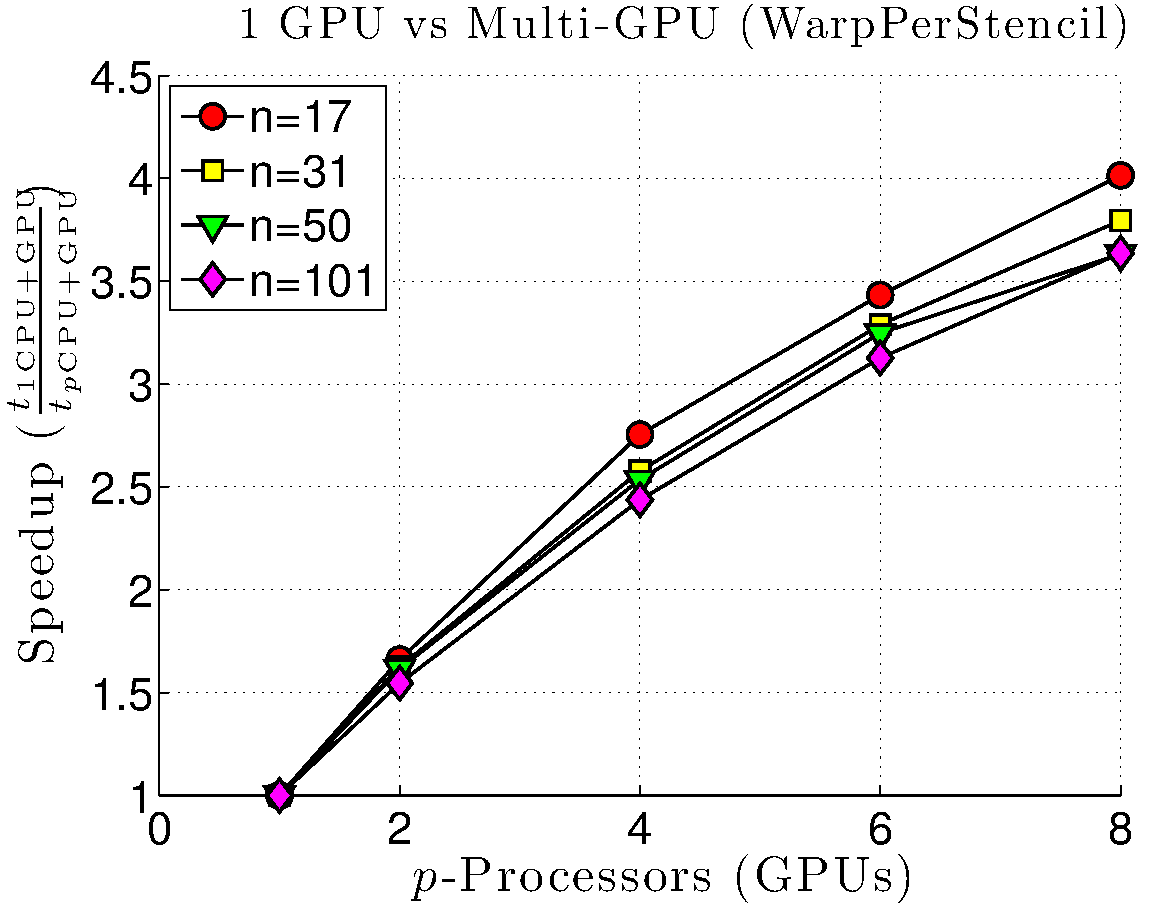
\includegraphics[width=1.0\textwidth]{../figures/spear_results/vortex/speedup_1GPU_vs_NGPU_WarpPerStencil-eps-converted-to.pdf}
\caption{Multi-GPU strong scaling vs one GPU on Spear for one warp per stencil}
\label{fig:spear_alltoall_multigpu_vs_gpu_scaling}
\end{subfigure} 
\caption{Distributed CPU and GPU scaling on the FSU Spear cluster.}
\end{figure} 




\section{Single GPU SpMV on Spear}

These results were run on Spear. MPI communication is done with an MPI\_alltoallv collective. The test case is the vortex roll-up. 

Figure~\ref{fig:spear_alltoall_1proc_warp} 

\begin{figure}
\centering
\begin{subfigure}[t]{0.425\textwidth}
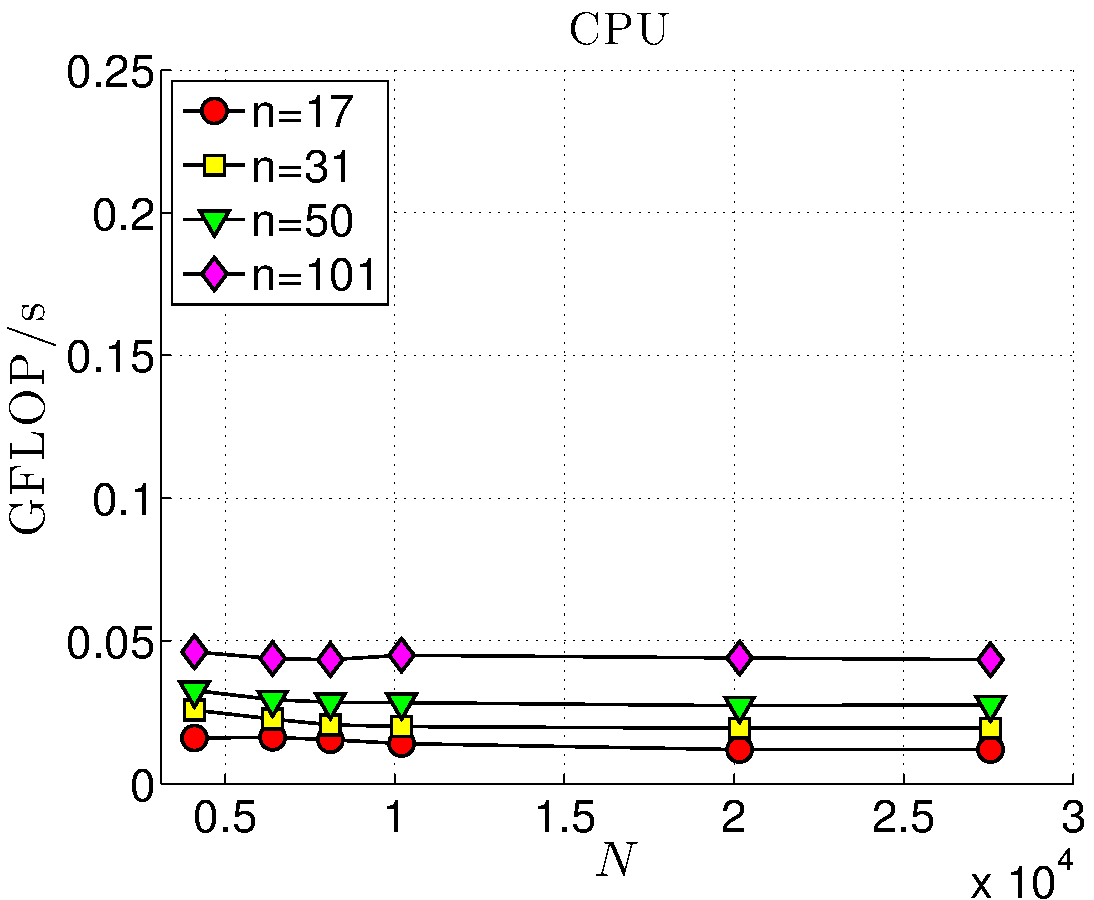
\includegraphics[width=1.0\textwidth]{../figures/spear_results/vortex/gflops_cpu_1proc_oneWarpPerStencil-eps-converted-to.pdf}
\caption{One warp per stencil kernel on one GPU in Spear \authnote{TODO: update} }
\label{fig:spear_alltoall_1proc_warp}
\end{subfigure} 

\begin{subfigure}[t]{0.425\textwidth}
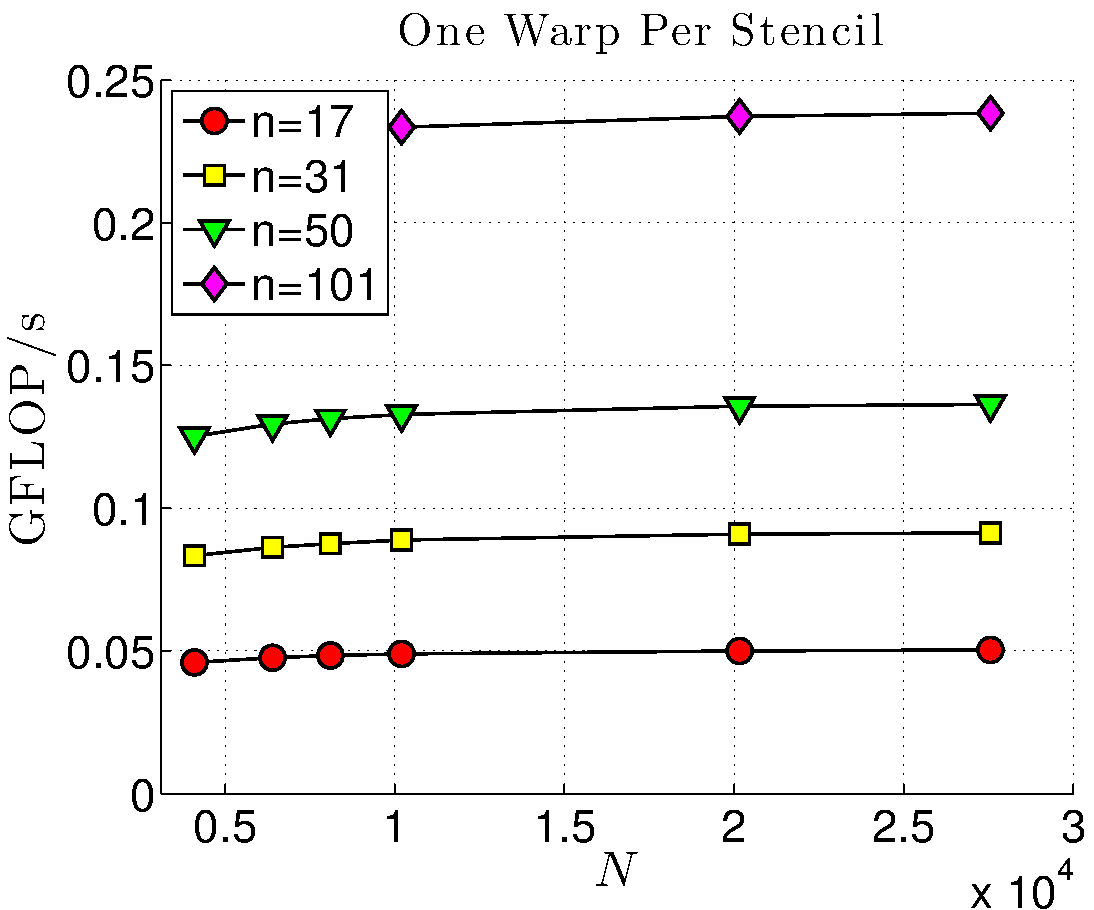
\includegraphics[width=1.0\textwidth]{../figures/spear_results/vortex/gflops_gpu_1proc_oneWarpPerStencil-eps-converted-to.pdf}
\caption{One warp per stencil kernel on one GPU in Spear}
\label{fig:spear_alltoall_1proc_warp}
\end{subfigure} 
\begin{subfigure}[t]{0.425\textwidth}
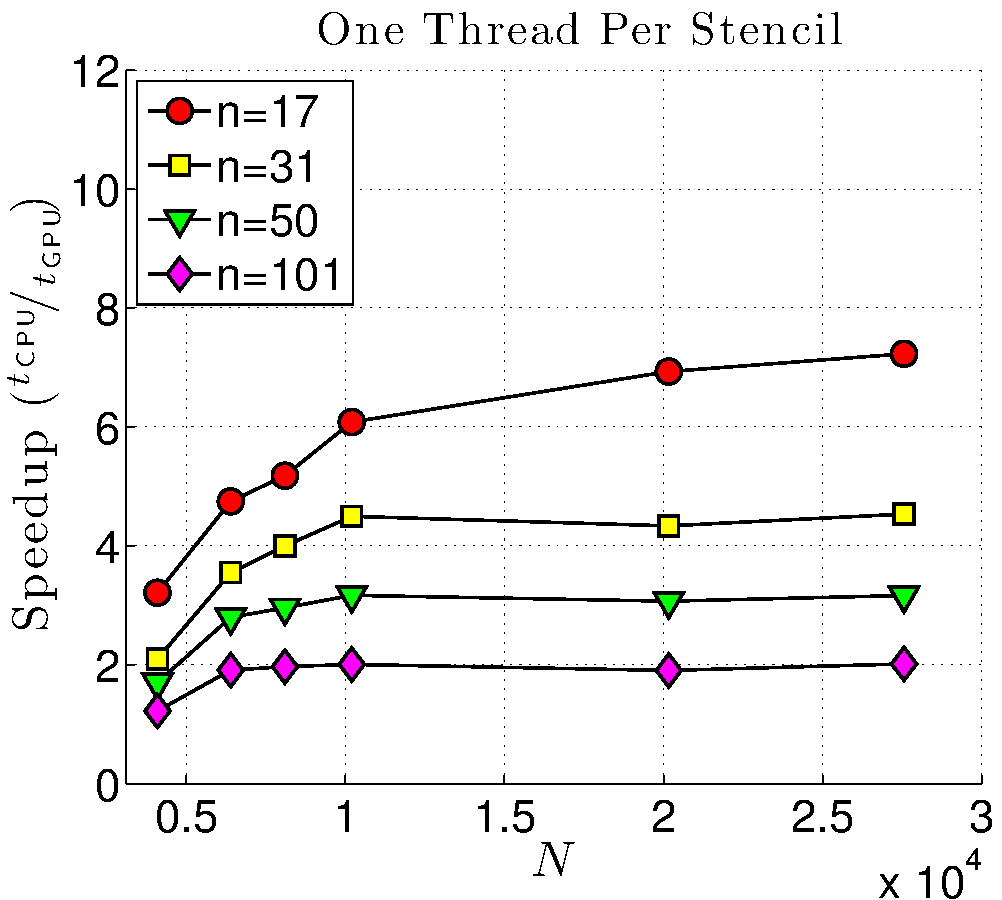
\includegraphics[width=1.0\textwidth]{../figures/spear_results/vortex/speedup_1proc_oneThreadPerStencil-eps-converted-to.pdf}
\caption{One warp per stencil kernel on one GPU in Spear}
\label{fig:spear_alltoall_1proc_warp}
\end{subfigure} 
\end{figure} 

\begin{figure}
\centering
\begin{subfigure}[t]{0.425\textwidth}
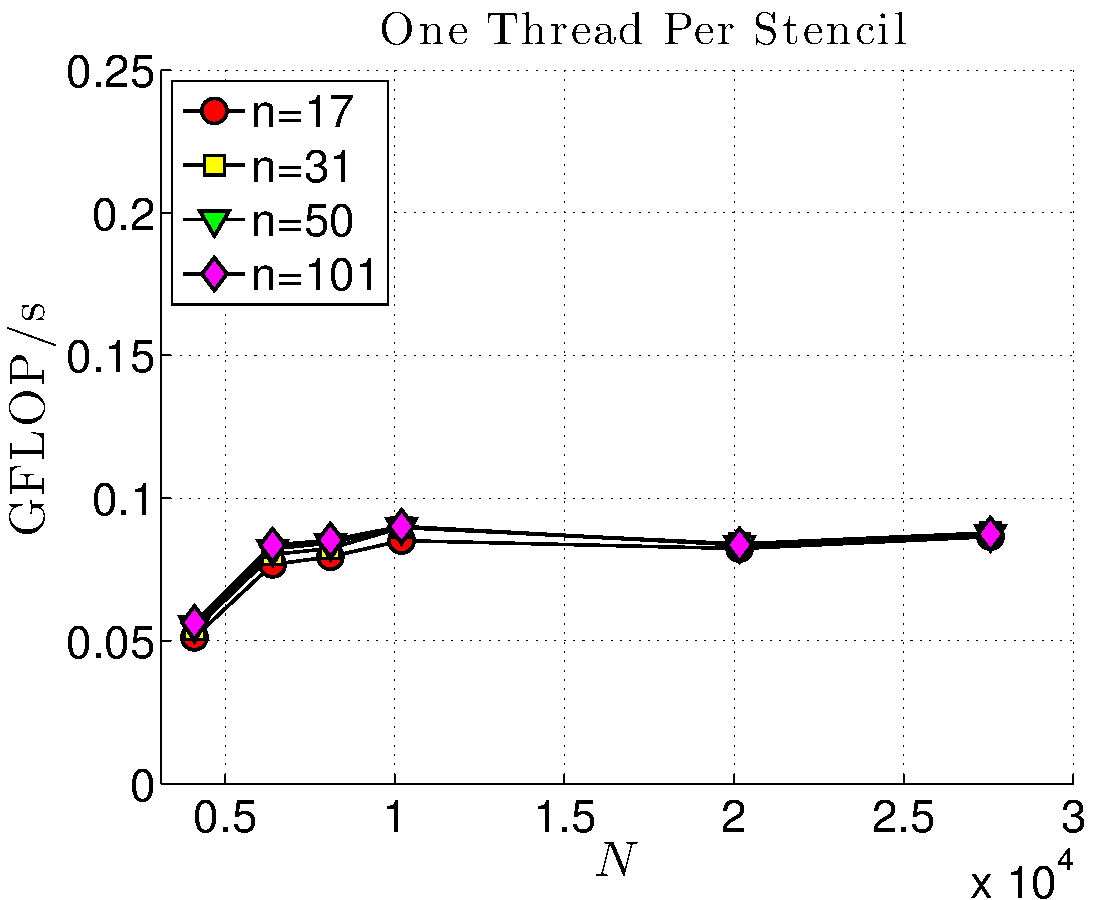
\includegraphics[width=1.0\textwidth]{../figures/spear_results/vortex/gflops_gpu_1proc_oneThreadPerStencil-eps-converted-to.pdf}
\caption{One warp per stencil kernel on one GPU in Spear}
\label{fig:spaer_alltoall_1proc_warp}
\end{subfigure} 
\begin{subfigure}[t]{0.425\textwidth}
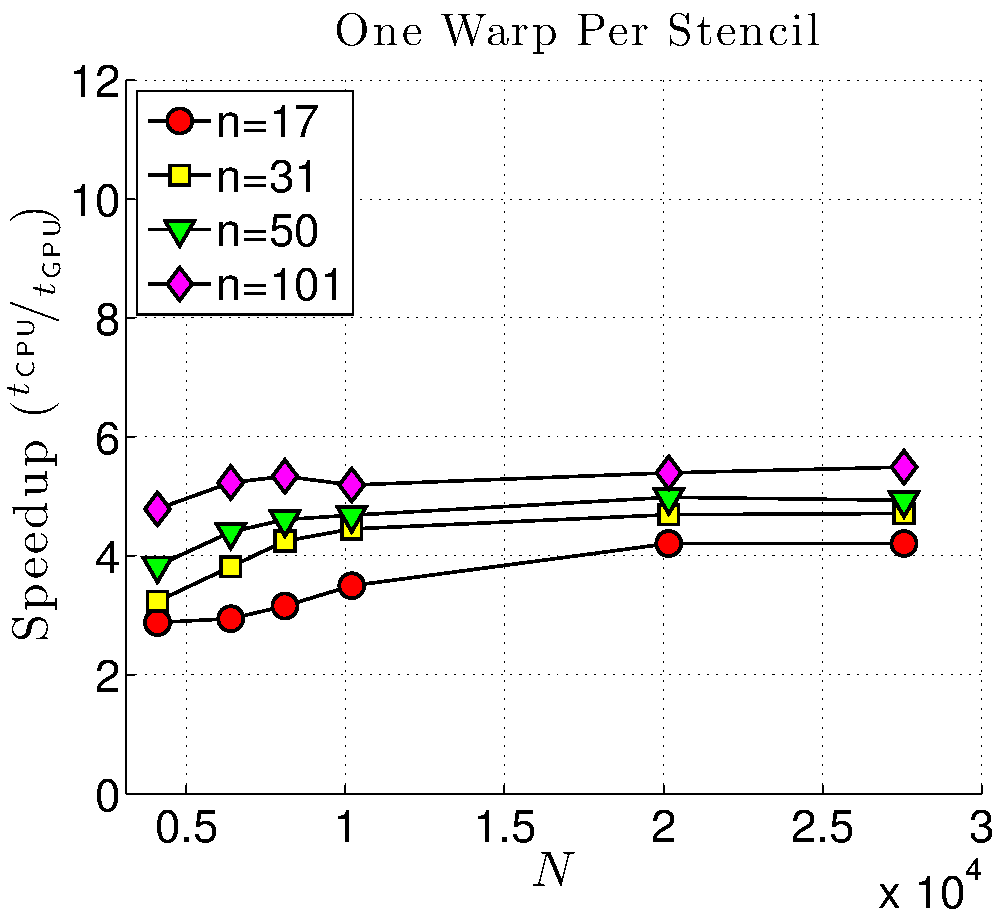
\includegraphics[width=1.0\textwidth]{../figures/spear_results/vortex/speedup_1proc_oneWarpPerStencil-eps-converted-to.pdf}
\caption{One warp per stencil kernel on one GPU in Spear}
\label{fig:spear_alltoall_1proc_warp}
\end{subfigure} 
\end{figure}

\section{ViennaCL}

These benchmarks compare performance of a single SpMV executed on Spear. Each data point is the average over 10 executions. The GPU is primed by an iteration before benchmarking begins. 

\begin{figure}
\centering
\begin{subfigure}[t]{0.48\textwidth}
\centering
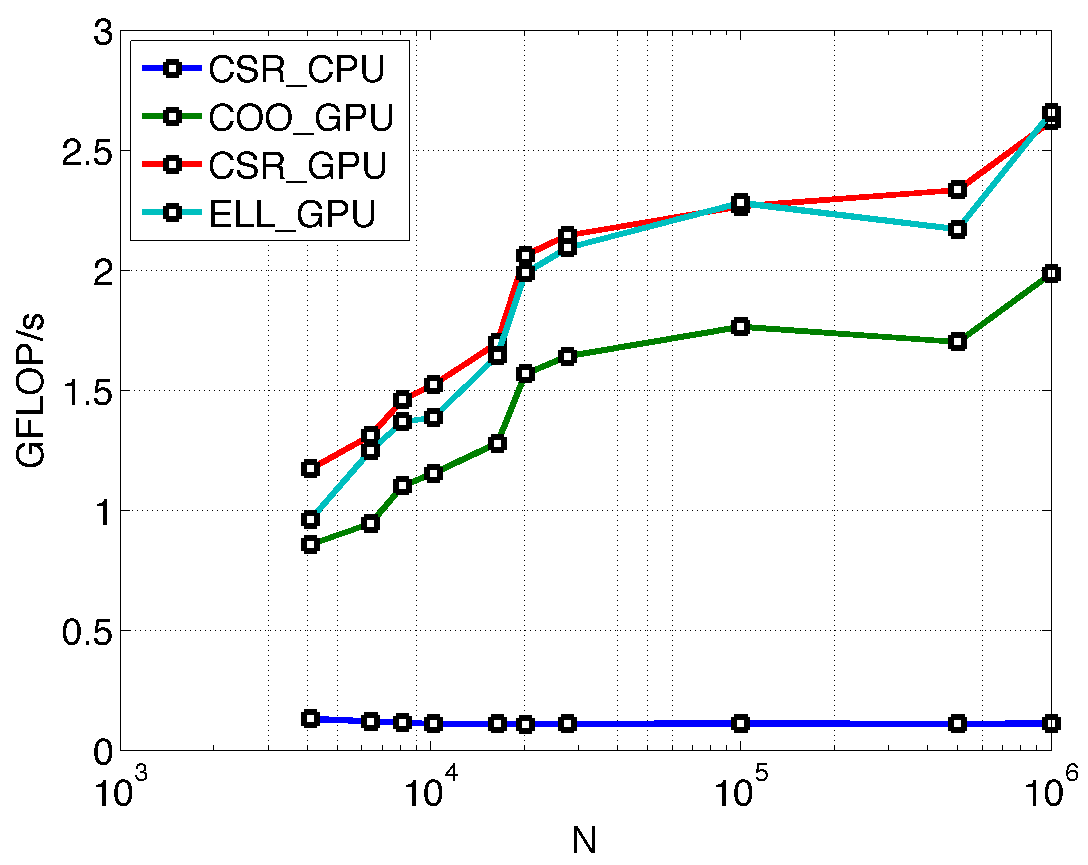
\includegraphics[width=1.0\textwidth]{../figures/spear_results/spmv/spmv_vcl_gflops-eps-converted-to.pdf}
\caption{SpMV Performance of the ViennaCL CSR, COO and ELL formats versus the BOOST::uBLAS CSR format.}
\label{fig:spear_vcl_gflops}
\end{subfigure} 
\begin{subfigure}[t]{0.48\textwidth}
\centering
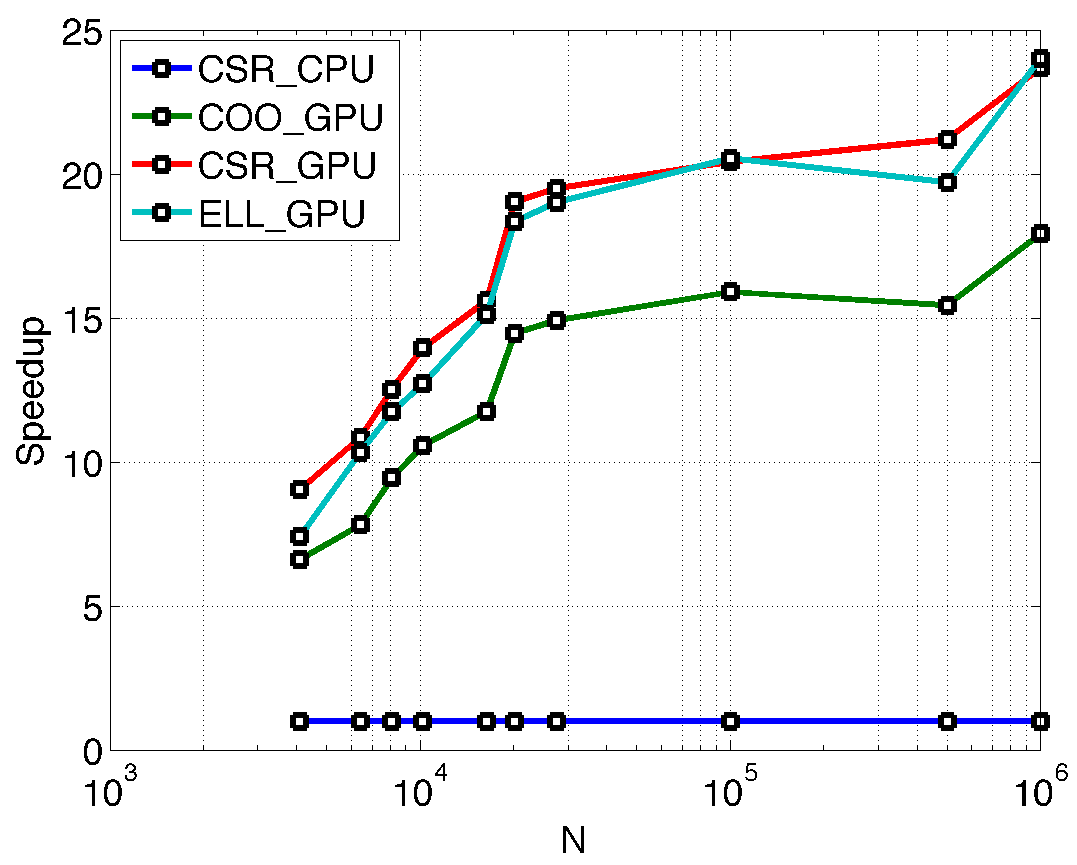
\includegraphics[width=1.0\textwidth]{../figures/spear_results/spmv/spmv_vcl_speedup-eps-converted-to.pdf}
\caption{Speedup relative to the BOOST::uBLAS CSR implementation on the CPU.}
\label{fig:spear_vcl_speedup}
\end{subfigure} 
\caption{Single GPU SpMV performance for ViennaCL vs BOOST::uBLAS on the Spear cluster (FSU) for $n=50$. }
\end{figure}




%I am generating another set of figures that demonstrate the scaling when we overlap communication and computation. MPI collectives do not allow overlap, but the asynchronous GPU kernel launches do. Therefore, I expect:
%    - the scaling on multiple CPUs vs 1 CPU to be the same as it is now
%    - the scaling on multiple GPUs vs 1 GPU will improve to linear/super-linear for problem sizes that occupy the hardware longer than the minimum kernel launch time. For N=27556 we might only see linear speedup up to 6 or 8 processors. 
%    - larger problem sizes will still be necessary (I have benchmarks for 100K, 500K and 1M on the sphere).
%    

%TODO: Work-Group Size and Number of Stencils
%What if a work-group is larger than a warp? What if the group was occupied by multiple stencils. What improvements to speedup do we see?
%
%How many stencils can each group handle (assuming values stay in shared memory? 
%Shared memory bank conflicts? How do we sort the values? 
%What is the occupancy of the GPU?
%

